\documentclass{article}
\usepackage{graphicx} % Required for inserting images
\usepackage{float}
\usepackage{hyperref}

\title{Supervised Machine Learning for Network Intrusion Detection Systems (NSL-KDD)}
\author{Omar Hyder - \href{https://github.com/OmarHyder07/ML-IDS}{GitHub repo}}
\begin{document}

\maketitle

\section{Summary}
I implemented logistic regression from scratch using NumPy to classify network connections as normal or anomalous on the NSL-KDD dataset. This is intended as a first baseline for an ML-based IDS. The model reaches $\mathbf{\sim96\%}$ training but only $\mathbf{\sim75\%}$ on the test set. This writeup argues that the gap is not overfitting in the usual sense but a consequence of distribution shift baked into NSL-KDD. 
\begin{center}
\begin{tabular}{ |c | c| } 
 \hline
 Metric (test set) & Value  \\
\hline 
 Accuracy & 0.75  \\ 
 Precision (anomaly) & 0.92  \\ 
 Recall (anomaly) & 0.62 \\
 F1 (anomaly) & 0.74 \\
 F2 (anomaly) & 0.66 \\
 \hline
\end{tabular}
\end{center}

\begin{figure}[H]
    \centering
    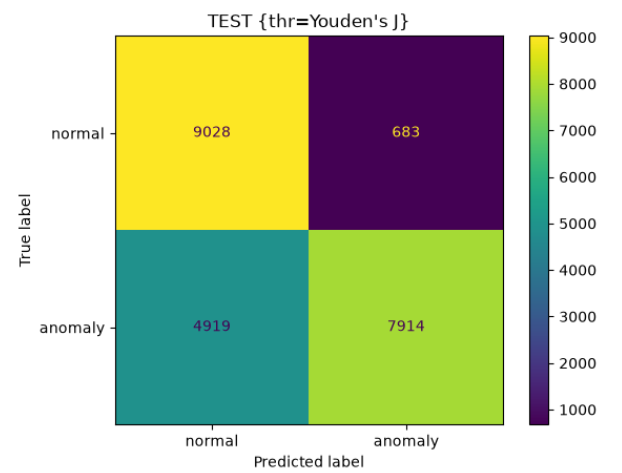
\includegraphics[width=0.7\linewidth]{Screenshot From 2026-07-20 20-06-55.png}
    \caption{Confusion matrix on test-set}
    \label{fig:placeholder}
\end{figure}


\section{Data Preparation}
\paragraph{Categorical Features}
\emph{protocol\_type}, \emph{service}, and \emph{flag} are unordered categories. Initially, I label-encoded them, then replaced this with one-hot encoding because label-encoding imposes a false ordinal scale. However, this change brought insubstantial gains, emphasising micro-optimisations in pre-processing was a dead end. Encoders were fit on training data only to avoid leakage.
\paragraph{Scaling}
First, I used standard scaling on all features. However, the \emph{src\_bytes} feature quickly caused overflow errors in my sigmoid function. Why? It and it's fellow byte-count feature \emph{dst\_bytes} are very, very heavy-tailed. Some values were $>$240 standard deviations from the mean, causing overflow and crushing 99\% of the data into an unusable sliver. This lead me to discovering the log transform, which is ideal for heavy-tailed data.
\paragraph{Challenges}
My loss was stuck at $\sim0.69$; ln(2). The loss of a coin-flip. How could a trained model be no better than a coin flip? Multiple calls to \emph{train\_test\_split} caused X and y to be shuffled - data and their associated labels were mismatched. Hours of model debugging could have been saved by more careful data-plumbing, hopefully a lesson I will carry into the future!
\begin{figure}[H]
    \centering
    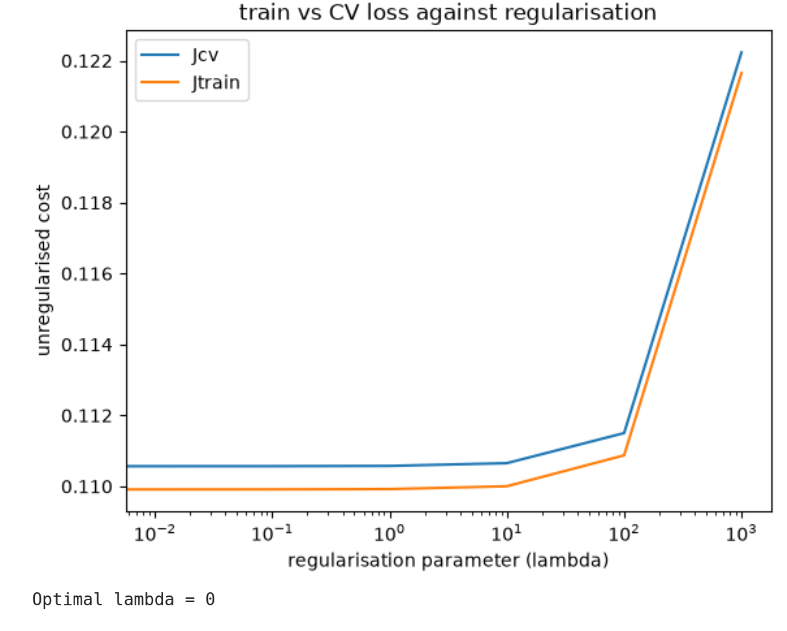
\includegraphics[width=1\linewidth]{Screenshot From 2026-07-20 19-44-09.png}
    \label{fig:placeholder}
\end{figure}
\section{Hyper-parameter Tuning}
I swept the L2 penalty across several orders of magnitude, comparing unregularised train and CV (taken from the training set, not test!) loss. The optimum was around 0; beyond which regularisation only increased CV loss. Train and CV loss being both low and near-identical showed me the model is not overfitting to the training set. Bad metrics were caused by something much more sinister...!

\section{Fitness of log-reg as an IDS}
\subsection{The core finding: distribution shift}
The 20 point train-test gap looks like high variance, but the regularisation study above shows the model generalises fine within the training distribution. The explanation is specific to this dataset: NSL-KDD's test set deliberately contains attack types not present in the training set. A supervised classifier cannot recognise attack families it has never seen, so a test-set ceiling exists that no amount of tuning on the training distribution can lift.
\paragraph{17 attack types in test but never in training}: 'httptunnel', 'xlock', 'xterm', 'sendmail', 'apache2', 'snmpgetattack', 'saint', 'xsnoop', 'named', 'worm', 'processtable', 'udpstorm', 'ps', 'sqlattack', 'mailbomb', 'mscan', 'snmpguess'
\begin{center}
\begin{tabular}{ |c | c| } 
 \hline
 Recall (seen attack types) & 0.714  \\
 Recall (novel attack types) & 0.380  \\ 
 \hline
\end{tabular}
\end{center}

\subsection{Conclusion}
For an IDS, a false negative (a missed attack) is far costlier than a false positive (a wasted analyst alert), so I selected the decision threshold to favour recall, using Youden's J on the CV set. Even so, test recall is only 0.62 — the model misses roughly a third of attacks — while keeping false positives low. The threshold chosen on CV did not fully transfer to the test set, itself a symptom of the distribution shift. Conclusion: this linear model is not adequate as an IDS. Its errors fall on exactly the novel attacks an IDS most needs to catch.
\paragraph{CIC-IDS2017} Looking forwards, for my flagship model trained on CIC-IDS2017, perhaps and unsupervised anomaly-detection approach (flagging deviation from "normal" rather than matching attack types) is the principled response to the distribution-shift problem. I am glad to have faced this on the training ground of NSL-KDD so as to know the reasonable direction to take next.
\begin{figure}[H]
    \centering
    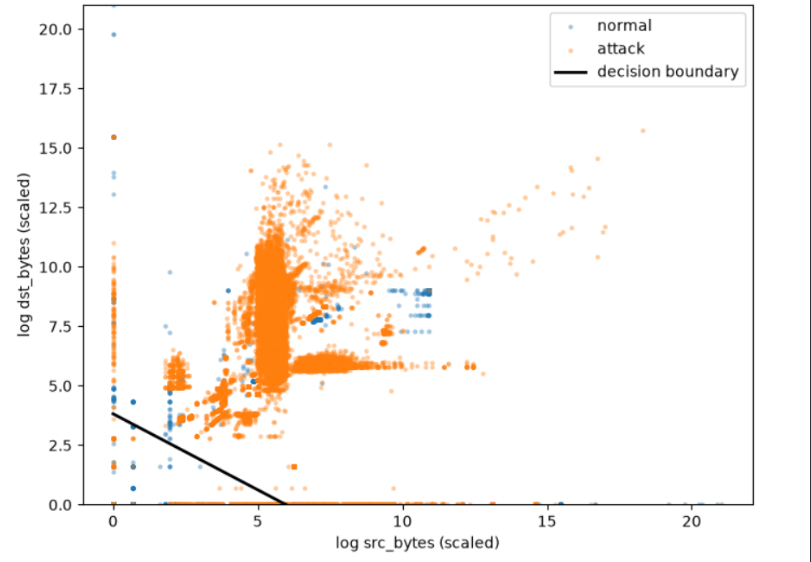
\includegraphics[width=0.8\linewidth]{Screenshot From 2026-07-20 20-10-29.png}
    \caption{dst\_bytes vs. src\_bytes with decision boundary}
    \label{fig:placeholder}
\end{figure}
\section{Trees: a more expressive supervised model}
Figure 2 above displays the fundamental simplicity of linear boundaries. Perhaps polynomial features would yield result, but at the cost of extreme compute (post encoding, there were 122 features). Decision trees and their ensembles are more expressive and may raise overall performance, but the distribution-shift ceiling should persist; the seen-vs-novel breakdown will tell us.
\paragraph{Which Tree model?} I trained a single Decision Tree, a Random Forest and an XGBoost classifier. The latter 2 had minimal hyper-parameter tuning. I did not believe the large compute time of using GridSearchCV would be worth it given that a highly tuned tree still faces the same distribution-shift issues logistic regression faced.
\begin{center}
\begin{tabular}{ |c | c| } 
 \hline
 Model & F2 (anomaly) \\
 \hline  
 Tree & 0.742  \\
 Random Forest & 0.648  \\ 
 XGBoost & 0.710 \\
 \hline
\end{tabular}
\end{center}
\paragraph{Novel recall} So, the seen-vs-novel split for a lone Decision Tree is as follows:
\begin{center}
\begin{tabular}{ |c | c| } 
 \hline
 Recall (seen attack types) & 0.784  \\
 Recall (novel attack types) & 0.502  \\ 
 \hline
\end{tabular}
\end{center}
A little better than logistic regression! But still only 0.2\% better than a coin flip. So no, more expressive supervised models are (most likely - maybe greater tuning would flip the script!) not suitable for an IDS.
\end{document}

